% Chapter 4 from the standard thesis template
%   that contains an adv. example table and figure.
\chapter{RESULTS}


This section reports the data collected throught the questionnaire in Qualtrics\textsuperscript{\textregistered}. All data is reported, including answers to open-ended questions. This chapter includes the current perceived knowledge of respondents in subjects related to carnivorous companion animal nutrition. Also included are data from numbered scale ratings on respondents knowledge of specific topics related to companion animal nutrition. Responses related to what types of nutritional education participants have taken part in and responses about personal opinions of different pet diets are also included. The chapter will end with results of open-ended questions.

\section{Identify Demographics}
This section shows data that contribute to the first two objectives of the study. There were respondents from almost every age range from 18 to over 66. The only age group with no respondents was the 36-45 year old age group. Most respondents were from the age range 18-25 with 36\% (\textit{n}=7) of responses in that range. There was a tie for the second highest response numbers at 21\% (\textit{n}=4) for age groups 26-35 and 56-65. Some respondents did not answer the demographic question of their current position. Only 63\% (\textit{n}=12) answered the question, and multiple answers were allowed. Veterinary technician students comprised 15\% (\textit{n}=3) of responses; one veterinary assistant responded (5\%), and 26\% (\textit{n}=5) responded that they are veterinary technicians. The rest of the responses were from veterinarians (\textit{n}=3) or people who fit into the ``other" category (\textit{n}=3). The vast majority of respondents owned cats or dogs, and some owned both; 63\% (\textit{n}=12) own dogs, 68\% (\textit{n}=13) own cats, and 5.3\% (\textit{n}=1) own neither. The number of dogs owned by respondents ranged from one to three with an average of 1.8 dogs per dog owner who participated. The minimum number of cats owned by respondents that own cats is one, and the maximum is fifteen barn cats; the average number of cats owned is 3.3 cats per participant who owns cats. As for the food that respondents' pets eat, multiple answers were allowed, but the majority of pet owners feed kibble at 83\% (\textit{n}=15). The other two types of foods respondents are giving their pets include canned or wet food at 17\% (\textit{n}=3) and homemade cooked or raw at 11\% (\textit{n}=2). Respondents are attending or attended a few different colleges, with the most respondents receiving their education from Muscatine Community College. Three respondents did not answer this question, leaving the total responses at sixteen for this question, 31\% (\textit{n}=5) of which attend or attended Muscatine Community College. The other responses were distributed between Des Moines Area Community College (\textit{n}=1), Hawkeye Community College (\textit{n}=2), Kirkwood Community College (\textit{n}=3), and four respondents selected the ``other" option and listed an unlisted college or university. All demographic data can be viewed in Table~\ref{tab:my_label}. Responses that listed ``other" will have the answer provided by the participant listed.

\begin{table}[htbp]
    \centering
    \caption{Demographic data for veterinary industry survey respondents}
    \label{tab:my_label}
    \begin{tabular}{c|c|cc}
    \hline
        &      &  \textit{f} & \% \\ \hline
    Age &  18-25   &  7 &   37  \\
        &  26-35   &  4 &   21  \\
        &  36-45   &  0 &   0   \\
        &  46-55    & 3 &   16  \\
        &  56-65    & 4 &   21  \\
        &   66+    &  1 &   5   \\  \hline
Position &  Veterinary Technician Student   &   3   &   15  \\
        &   Veterinary Assistant    &   1   &   5   \\
        &   Veterinary Technician   &   5   &   26  \\
        &   Veterinarian    &   3   &   25  \\
        &   Hospital Administrator  &   1   &   5   \\
        &   Office Manager  &   1   &   5   \\
        &   Other(unspecified)  &   1   &   5   \\
        &   No Response &   7   &   37  \\  \hline
Pet Ownership   &   Dog &   12  &   63  \\
        &   Cat &   13  &   68  \\
        &   None    &   1   &   5   \\  \hline
Number of Dogs     &   1   &   5   &   42  \\
        &   2   &   4   &   33  \\
        &   3   &   3   &   25  \\  \hline
Number of Cats     &   1   &   5   &   38  \\
        &   2   &   3   &   23  \\
        &   3   &   2   &   15  \\
        &   5   &   1   &   8   \\
        &   6   &   1   &   8   \\
        &   15  &   1   &   8   \\ \hline
Primary diet    &   Kibble  &   15  &   83  \\
        &   Canned or Wet   &   3   &   17  \\
        &   Home-Prepared Cooked or Raw &   2   &   11  \\  \hline
College Attending or Attended   &   Des Moines Area Community College   &   1   &   5   \\
        &   Muscatine Community College &   5   &   26  \\
        &   Hawkeye Community College   &   2   &   10  \\
        &   Kirkwood Community College  &   3   &   16  \\
        &   Mount Mercy University  &   1   &   5   \\
        &   Texas A\&M University   &   1   &   5   \\
        &   University of Missouri  &   1   &   5   \\
        &   Iowa State University   &   1   &   5   \\
        &   No Response &   3   &   16  \\  \hline
    \end{tabular}
\end{table}

\section{Identify differences in opinion between groups}
First, because only one respondent was not a pet owner, there is not enough data for results to be significant. Based on the one participant who does not own a pet, there is no significant difference in knowledge or opinion purely based on pet ownership, but this is not conclusive to any degree. Based on a cross tabulation between current position and opinions on whether companion animal nutrition courses should be available to all students in these programs of study, there is no difference in responses based on position. In the same cross tabulation, there seems to be no significant difference in opinion about different diets, although, the table looks more dispersed for responses in the groups currently working in veterinary clinics. Figure~\ref{mgraph} shows the cross tabulation, where it can be seen there is no obvious pattern of responses between groups based on position or student status. There also appears to be no significant difference in opinion across age groups, as can be seen from the distribution in Figure~\ref{mgraph2}. The only two respondents that did not say affirmatively that students should have the option to take companion animal nutrition courses in their community college program were on the younger side of the age range.

    \begin{figure}[htbp] \centering
    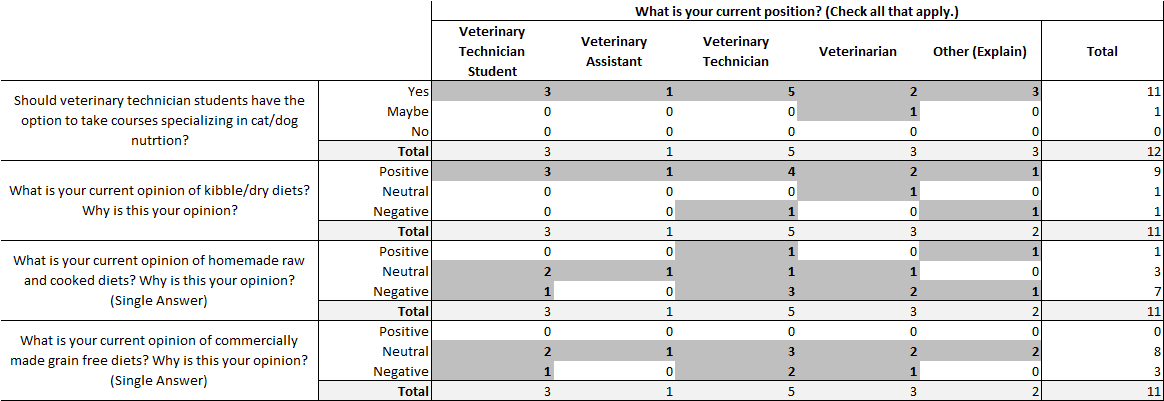
\includegraphics[width=1.3\textwidth, angle=90]{Images/Crosstab1.png}
    \isucaption{Cross Tabulation of Opinion Questions with Position}
    \label{mgraph}
    \end{figure}
    \begin{figure}[htbp] \centering
    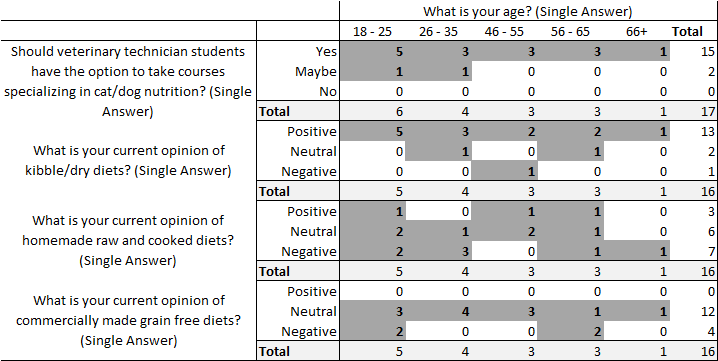
\includegraphics[width=1.1\textwidth, angle=90]{Images/Crosstab2.png}
    \isucaption{Cross Tabulation of Opinion Questions with Age}
    \label{mgraph2}
    \end{figure}
    
\section{Identify knowledge level in students}
Since only students had access to the survey early on in the collection period, the responses used for this objective were filtered by completion date since some respondents did not answer the student status question. There were ten responses filtered out through this method, but only 9 students finished the survey and answered this question. Those nine students rated their current knowledge of carnivorous companion animal nutrition at a 6.2 on average. The range was 3 to 9.1 with a median of 7. The scale used was a 1 to 10 scale where 1 was novice and 10 was expert. The average and median suggest that these students are fairly knowledgeable in the area of dog and cat nutrition, though there are a few who do not perceive themselves to be very knowledgeable. The spread of responses can be seen in Figure~\ref{mgraph3}.
    \begin{figure}[htbp] \centering
    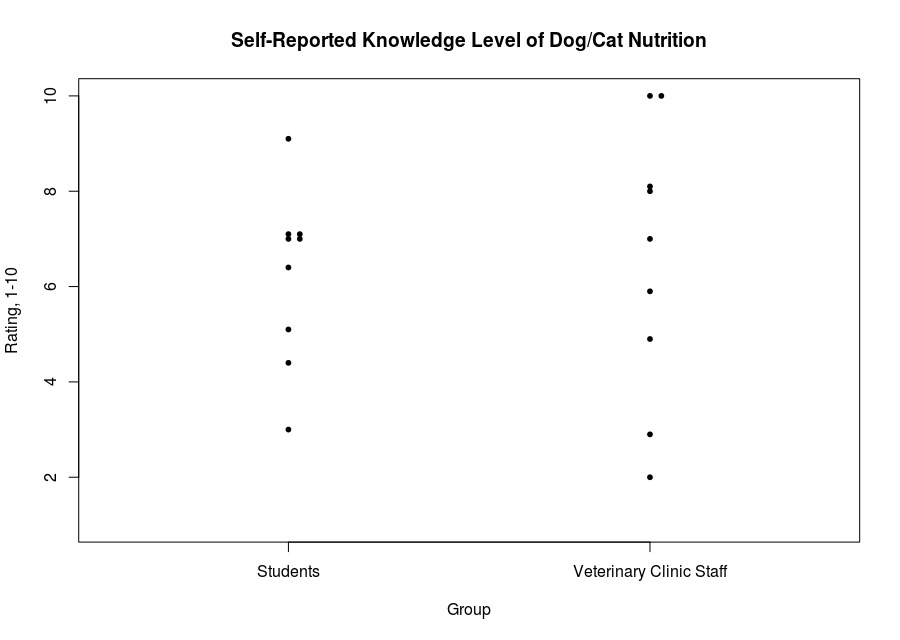
\includegraphics[width=1.0\textwidth]{Images/srkl.jpeg}
    \isucaption{Self-Reported Knowledge Level of Dog/Cat Nutrition}
    \label{mgraph3}
    \end{figure}
\par Based on the scale ratings of knowledge level in specific topics related to companion animal nutrition, the students seem to feel knowledgeable in many of the basic areas of companion animal nutrition. The data can be seen in Figure~\ref{mgraph4} and Figure~\ref{mgraph12} which shows the average rating with each topic in small animal nutrition. The scale used was a 1 to 10 scale where 1 was not knowledgeable at all and 10 was extremely knowledgeable. The range of average ratings was 3.3 to 7.1. The following topics had an average rating higher than 5: canned and wet food advantages and disadvantages, kibble diet advantages and disadvantages, diet formulation, digestive physiology, digestive anatomy, ingredients, regulations and labeling, pet food labels, and clinical nutrition. The subjects which had an average rating below a 5 include the following: commercial refrigerated or raw formulations, homemade diet formulation, either raw or cooked, and freeze-dried foods. The student knowledge related to history of the pet food industry averages to equal 5. None of the averages were above 8.
    \begin{figure}[htbp] 
    \centering
    \textbf{How Knowledgeable Students are in Nutrition Topics (Averages)}\par\medskip
    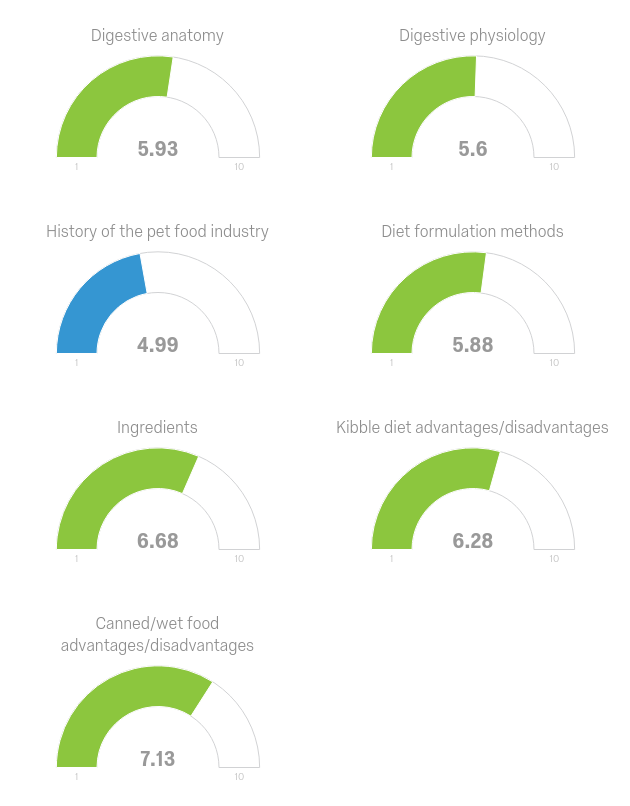
\includegraphics[width=0.9\textwidth]{Images/nks.png}
    \isucaption{Each arch graphic represents a scale from 1 to 10 for knowledge level. 1 = not knowledgeable; 10 = extremely knowledgeable. The number associated with each graphic is the average knowledge rating for that subject.}
    \label{mgraph4}
    \end{figure}
    \begin{figure}[htbp] 
    \centering
    \textbf{How Knowledgeable Students are in Nutrition Topics (Averages)}\par\medskip
    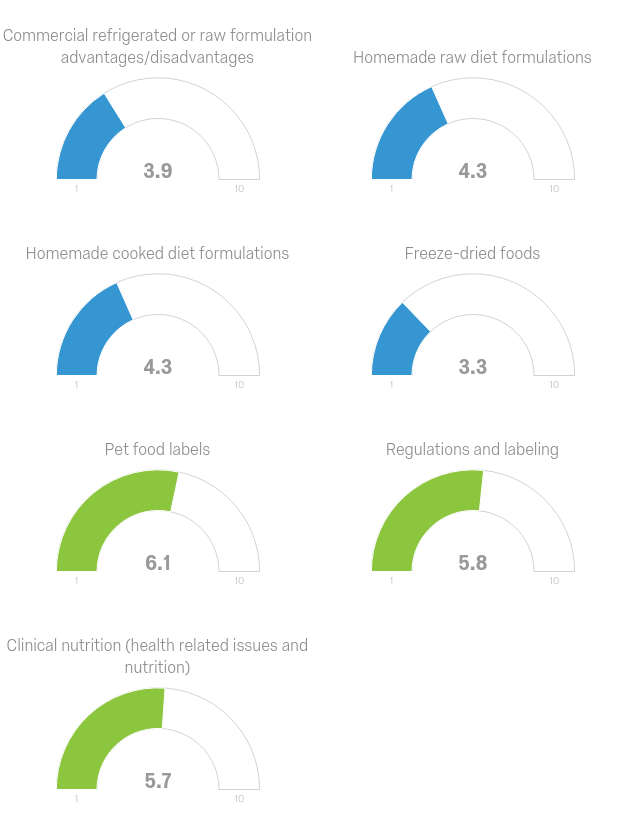
\includegraphics[width=0.9\textwidth]{Images/nks2.png}
    \isucaption{Each arch graphic represents a scale from 1 to 10 for knowledge level. 1 = not knowledgeable; 10 = extremely knowledgeable. The number associated with each graphic is the average knowledge rating for that subject.}
    \label{mgraph12}
    \end{figure}
\par The knowledge students possess of various pet food brands varies more significantly than the knowledge of topics in small animal nutrition. The average familiarity with specific pet food brands ranged from 1.6 for Nutrisca to 7.4 for Science Diet. The scale used was a 1 to 10 scale where 1 was not familiar at all, and 10 was extremely familiar. Nutrisca, Castor \& Pollux, Orijen, and Solid Gold all had average familiarity ratings below 2.5. Nutro, Royal Canin, Nature's Variety, Fromm, Nature's Recipe, and Diamond all had familiarity ratings between 2.5 and 5. Science Diet, Purina Dog or Cat Chow, Purina ProPlan, Pedigree, Iams, and Blue Buffalo all had ratings above 5, but none of the averages was above 8. Figure~\ref{mgraph5} shows the data in a way to easily compare the average ratings of pet foods with one another.
    \begin{figure}[htbp] 
    \centering
    \textbf{How Familiar Students are with Pet Food Brands (Averages)}\par\medskip
    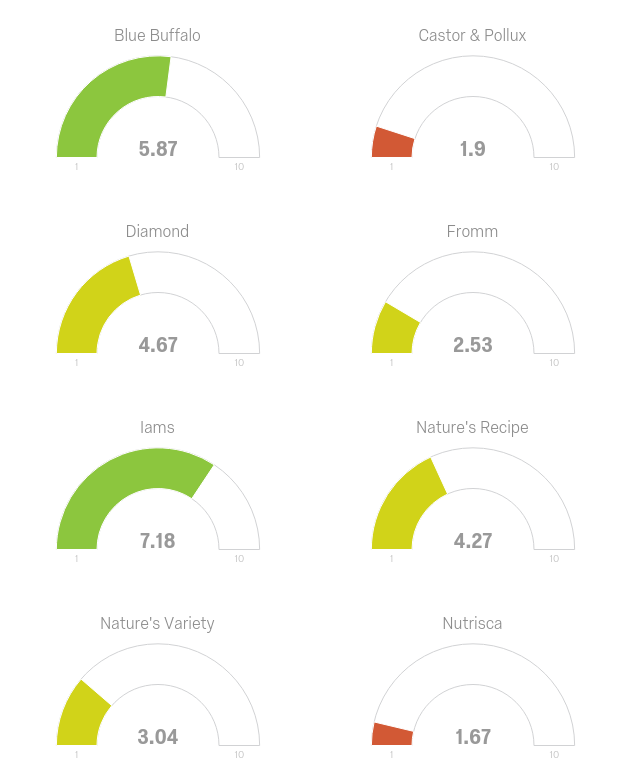
\includegraphics[width=0.9\textwidth]{Images/pffs.png}
    \isucaption{Each arch graphic represents a scale from 1 to 10 for familiarity. 1 = not familiar; 10 = extremely familiar. The number associated with each graphic is the average familiarity rating for that pet food brand.}
    \label{mgraph5}
    \end{figure}
    \begin{figure}[htbp] 
    \centering
    \textbf{How Familiar Students are with Pet Food Brands (Averages)}\par\medskip
    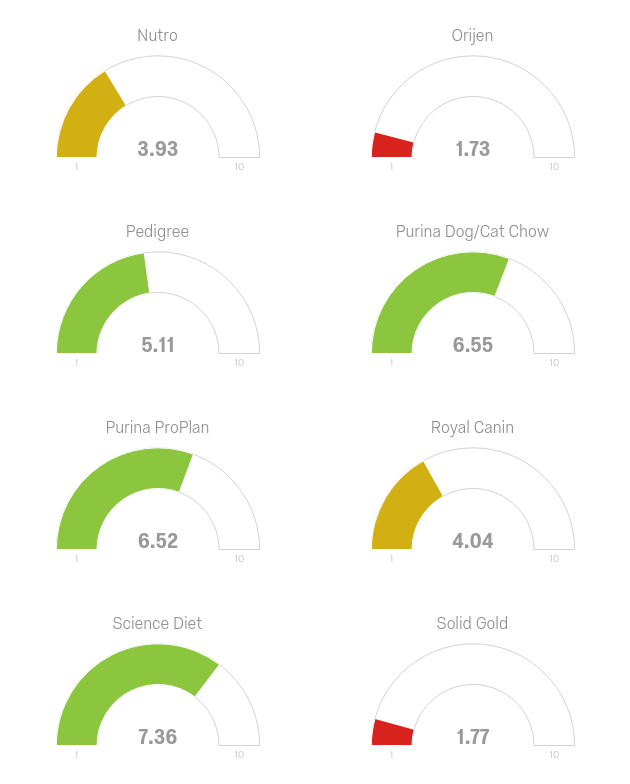
\includegraphics[width=0.9\textwidth]{Images/pffs2.png}
    \isucaption{Each arch graphic represents a scale from 1 to 10 for familiarity. 1 = not familiar; 10 = extremely familiar. The number associated with each graphic is the average familiarity rating for that pet food brand.}
    \label{mgraph13}
    \end{figure}
\section{Identify the interest level in an educational program}
All participants were asked of their interest in an educational program on nutrition because the researchers want to find out if there is a need overall. Since anyone can enroll in a community college to take a class they are interested in, there is the potential for graduates currently working in the industry to go back to take a course if they are interested. The average interest rating in an educational program designed for further learning in carnivorous companion animal nutrition was an 8.2, and the median was an 8.1 on a scale of 1 to 10 where 1 is not interested at all, and 10 is extremely interested. The range of responses was 3.4 at the lowest and 10 at the highest. The distribution is shown in Figure~\ref{mgraph6} where it may be suggested that the response of 3.4 is an outlier, even with the small sample size because the next lowest rating is 6.9. This is not conclusive, however, as the sample size is too small to definitively identify outliers.
    \begin{figure}[htbp] 
    \centering
    \textbf{}\par\medskip
    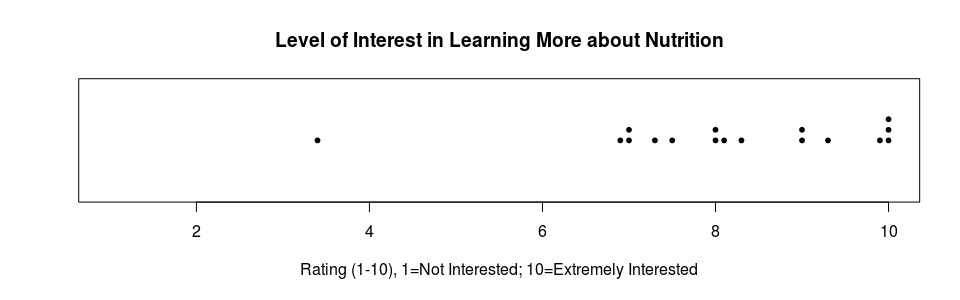
\includegraphics[width=1.0\textwidth]{Images/loiilman.jpeg}
    \isucaption{Each dot represents one participant's level of interest in learning more about companion animal nutrition.}
    \label{mgraph6}
    \end{figure}
\section{Identify perceptions of different diet philosophies}
For the questions asking the opinions of participants related to pet food diets, there were 16 respondents as 3 respondents discontinued the survey before seeing these questions. Most participants have a positive opinion of kibble diets overall. Two are neutral, and one participant has a negative opinion of kibble diets. The reasons for these opinions vary; this participant has a positive opinion of kibble foods and states the following as his or her reason:
\begin{quote}
``My dog has been on a dry diet his whole life and has been very healthy."
\end{quote}
Other participants with positive opinions of kibble diets state more specific reasons like the following:
\begin{quote}
``for texture, crunch, and to aid in cleaning teeth"
\end{quote}
\begin{quote}``I think they are the better option for most people because they provide a balanced diet and keep for longer periods of time"
\end{quote}
One of the participants with a neutral opinion of kibble diets thinks these diets are okay for dogs, but recommends a canned diet for cats due to higher moisture content and fewer carbohydrates. The participant who has a negative opinion of kibble diets prefers a fresh food diet for pets. Numerical data for the responses to the opinion question on kibble can be viewed in Table~\ref{tab:my_label2}
\par The opinions of homemade cooked and raw diets are very mixed. This question on diet opinion was the most varied among participants' answers. The distribution of responses was more even than with the other two questions on diet opinions. Three participants have positive opinions of homemade diets, six are neutral about them, and seven participants have negative opinions of homemade pet diets. One of the respondents with a positive opinion stated this as his or her reasoning:
\begin{quote}
``My 19 yr old cat was failing, throwing up dry and canned food. Now I cook or feed raw. Gained wt. no throwing up, shiny coat and SCREAMS for meat."
\end{quote}
This respondent is using personal experience for the reasoning behind the positive opinion of homemade diets. Some respondents were very neutral about homemade diets because they haven't used them or do not know enough to have an opinion. There was somewhat of a theme or two among reasons for negative opinions of homemade diets as is seen in the following:
\begin{quote}
``nutritional value; E.coli and Salmonella: they aren't wolves in the wild."
\end{quote}
\begin{quote}
``Most homemade diets are not properly balanced unless formulated by a vet nutritionist. Raw diets carry risks of bacterial contamination for both the animal and humans in the household, and do not have any proven benefits."
\end{quote}
The rest of the reasons in each opinion category are similar to the responses included. The number of responses for each opinion option are displayed in Table~\ref{tab:my_label2}.
\par Lastly, the opinions of participants in the area of commercial grain free pet diets is mostly neutral. Twelve respondents were neutral about grain free diets, while four had negative opinions about commercially made grain free pet food. No respondents were positive about this type of diet. However, some of the reasons show that some respondents do have positive experiences with grain free foods. Two respondents who are neutral about grain free foods said the following:
\begin{quote}
``I had a cat who was particularly allergic to something in a diet that had grains. Went to grain free and her allergies disappeared. I do believe it is not necessary for the majority of animals and overly advertised."
\end{quote}
\begin{quote}
``Great for those animals that are sensitive to cereal grains"
\end{quote}
Other neutral responses had a different tone such as this reason:
\begin{quote}
``I think it's just hype"
\end{quote}
Some of the responses showing negative opinions were obviously more opinionated about the grain free diets than others, such as this respondent:
\begin{quote}
````Grain Free" (notice the quotes) is a fad with little if any scientific basis."
\end{quote}
The data showing how many responses were received for each choice in the grain free opinion question is shown with the previous data in Table~\ref{tab:my_label2}

\begin{table}[h!]
    \centering
    \caption{Participant opinions of different pet diets}
    \label{tab:my_label2}
    \begin{tabular}{c|c|cc}
    \hline
            &      &  \textit{f} & \% \\ \hline
    Kibble  &   Positive    &   13  &   81  \\
            &   Neutral     &   2   &   12  \\
            &   Negative    &   1   &   6   \\  \hline
    Homemade Raw and Cooked &   Positive    &   3   &   19  \\
            &   Neutral     &   6   &   38  \\
            &   Negative    &   7   &   44  \\  \hline
    Commercial Grain Free   &   Positive    &   0   &   0   \\
            &   Neutral     &   12  &   75  \\
            &   Negative    &   4   &   25  \\  \hline
  \end{tabular}
\end{table}        

\section{Identify knowledge level in veterinary staff}
A filter based on survey start date was used since only veterinary staff was given access after a certain point in survey collection. There were nine responses filtered out this way, and those nine responses had an average perceived knowledge level of 7.5 with a median of 7.1 and a range from 3 to 10. The scale used was a 1 to 10 scale where 1 was novice and 10 was expert. These numbers are pretty similar to the knowledge level numbers of students listed above. The distribution of these answers can be seen in Figure~\ref{mgraph3}.
\par The knowledge level of veterinary staff in the topics related to companion animal nutrition seems to be generally higher than that of the students. The scale used was a 1 to 10 scale where 1 was not knowledgeable at all and 10 was extremely knowledgeable. The highest rating average is 8.3 for two topics in small animal nutrition, and the lowest is 4.1. The categories where respondent rating average was 8 or higher included clinical nutrition, pet food labels, canned and wet food advantages and disadvantages, and kibble advantages and disadvantages. The categories where respondent rating averaged between 5 and 8 were digestive anatomy, digestive physiology, history of the pet food industry, diet formulation methods, ingredients, regulations and labeling, and commercial refrigerated or raw advantages and disadvantages. Categories with average ratings below 5 included homemade raw diet formulations, homemade cooked diet formulations, and freeze-dried foods. The charts comparing the average rating for these categories can be viewed in Figure~\ref{mgraph8} and Figure~\ref{mgraph14}.
    \begin{figure}[htbp] 
    \centering
    \textbf{How Knowledgeable Clinic Staff are in Nutrition Topics (Averages)}\par\medskip
    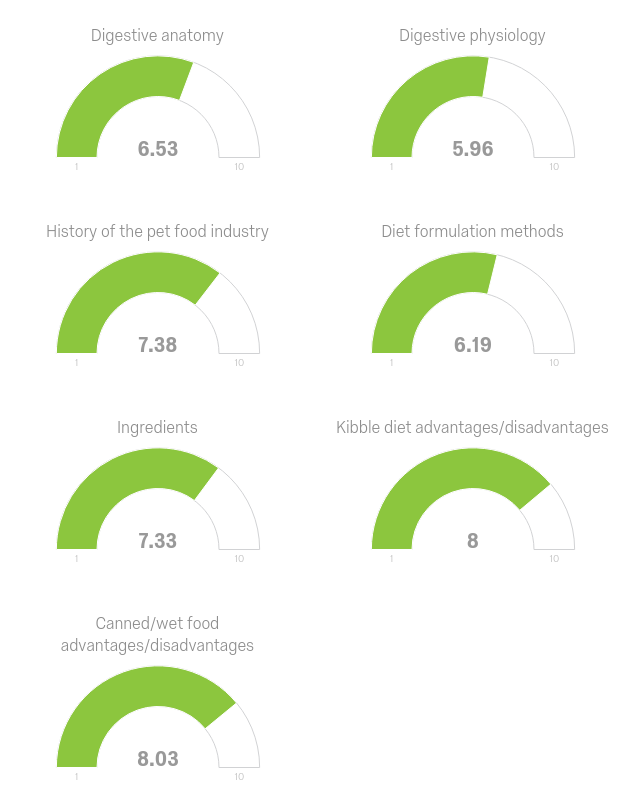
\includegraphics[width=0.9\textwidth]{Images/nkcs.png}
    \isucaption{Each arch graphic represents a scale from 1 to 10 for knowledge level. 1 = not knowledgeable; 10 = extremely knowledgeable. The number associated with each graphic is the average knowledge rating for that subject.}
    \label{mgraph8}
    \end{figure}
    \begin{figure}[htbp] 
    \centering
    \textbf{How Knowledgeable Clinic Staff are in Nutrition Topics (Averages)}\par\medskip
    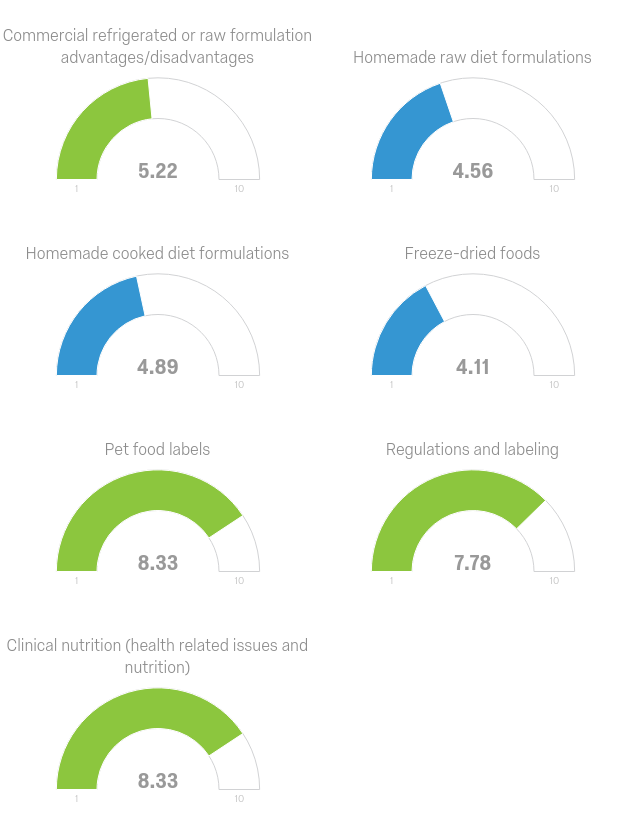
\includegraphics[width=0.9\textwidth]{Images/nkcs2.png}
    \isucaption{Each arch graphic represents a scale from 1 to 10 for knowledge level. 1 = not knowledgeable; 10 = extremely knowledgeable. The number associated with each graphic is the average knowledge rating for that subject.}
    \label{mgraph14}
    \end{figure}
\par The familiarity level of veterinary staff in pet food brands differs from the knowledge levels in the categories of pet nutrition. The scale used was a 1 to 10 scale where 1 was not familiar at all and 10 was extremely familiar. The range of rating average is significantly wider, from a low of 1.7 to a high of 9.1. The pet food that was most familiar, with an average rating above 8 was Science Diet, with an average rating of 9.1. The pet foods that were fairly familiar among veterinary staff, where the average rating was between 5 and 8, included Iams, Pedigree, Purina Dog and Cat Chow, Purina ProPlan, and Royal Canin. The less well-known brands, with average ratings between 2.5-5, are Solid Gold, Nutro, Orijen, Blue Buffalo, Diamond, Fromm, Nature's Recipe, and Nature's Variety. Two brands, Nutrisca and Castor \& Pollux, were very unfamiliar with a rating below 2.5. The graphic showing the comparison between the average ratings of different brands can be seen in Figure~\ref{mgraph9} and Figure~\ref{mgraph15}.
    \begin{figure}[htbp] 
    \centering
    \textbf{How Familiar Clinic Staff are with Pet Food Brands (Averages)}\par\medskip
    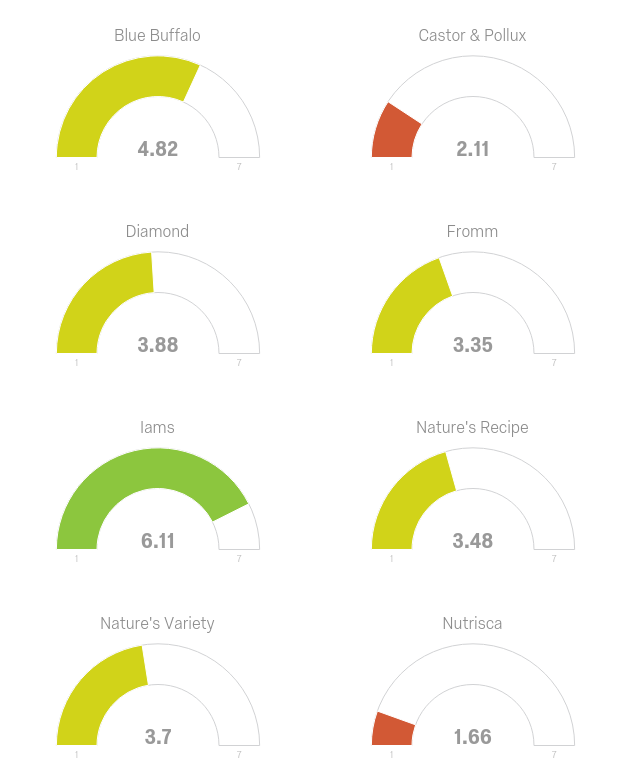
\includegraphics[width=0.9\textwidth]{Images/pffcs.png}
    \isucaption{Each arch graphic represents a scale from 1 to 10 for familiarity. 1 = not familiar; 10 = extremely familiar. The number associated with each graphic is the average familiarity rating for that pet food brand.}
    \label{mgraph9}
    \end{figure}
    \begin{figure}[htbp] 
    \centering
    \textbf{How Familiar Clinic Staff are with Pet Food Brands (Averages)}\par\medskip
    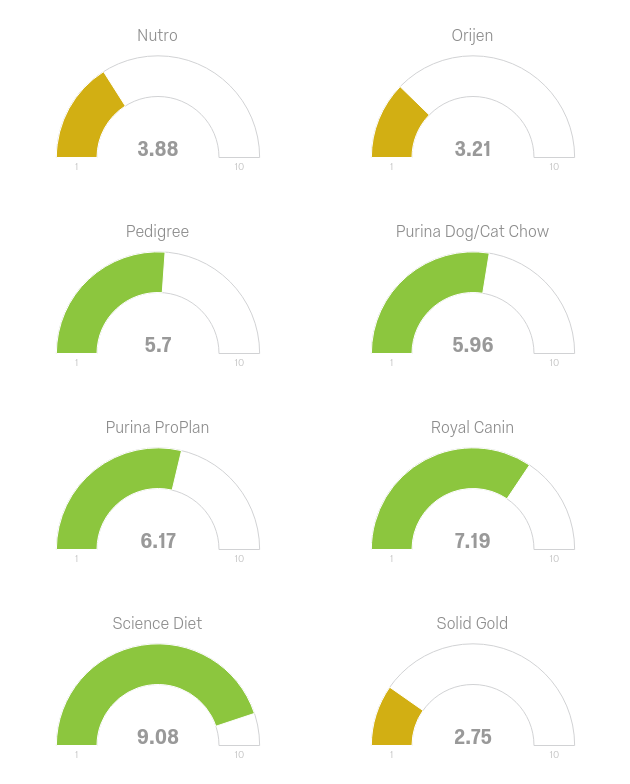
\includegraphics[width=0.9\textwidth]{Images/pffcs2.png}
    \isucaption{Each arch graphic represents a scale from 1 to 10 for familiarity. 1 = not familiar; 10 = extremely familiar. The number associated with each graphic is the average familiarity rating for that pet food brand.}
    \label{mgraph15}
    \end{figure}
\section{Identify value and importance of unbiased education}
First, the importance of veterinary staff with a strong nutritional background was rated by respondents. All 19 respondents answered this question and resulted in an average of 7.8 on a scale of 1 to 10 where 1 was not important at all and 10 was extremely important. The range of answers was from 1.9 to 10, and the median was 8. Out of the 19 responses, 11 respondents rated the importance 8 or higher, with 6 of those ratings being 10. The grouping of responses is fairly one-sided with all except two responses above a rating of 5. The distribution of ratings suggests an strong background in nutrition is fairly to very important to veterinary clinics. The distribution of ratings can be seen in Figure~\ref{mgraph10}.
    \begin{figure}[htbp] 
    \centering
    \textbf{Importance of Veterinary Staff Possessing Strong Nutritional Background}\par\medskip
    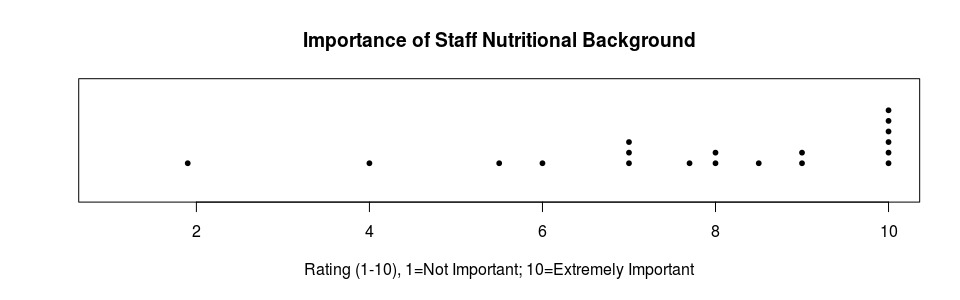
\includegraphics[width=1.0\textwidth]{Images/iosnb.jpeg}
    \isucaption{Each dot represents one participant's rating of importance.}
    \label{mgraph10}
    \end{figure}
\par Next, the value of unbiased carnivorous companion animal nutrition education was rated by participants. Seventeen of the 19 respondents answered this question, resulting in an average of 8.2 on a scale of 1 to 10 where 1 was not valuable at all, and 10 was extremely valuable. The range of answers was from 5 to 10, and the median was 9. Out of the 17 responses, 12 respondents rated the value at 8 or higher, with 4 of the ratings being 10. All ratings were above a 5, showing strong support for unbiased education being fairly to very valuable in a veterinary technician or assistant. The distributions of responses for value of unbiased education can be viewed in Figure~\ref{mgraph11}.
    \begin{figure}[htbp] 
    \centering
    \textbf{}\par\medskip
    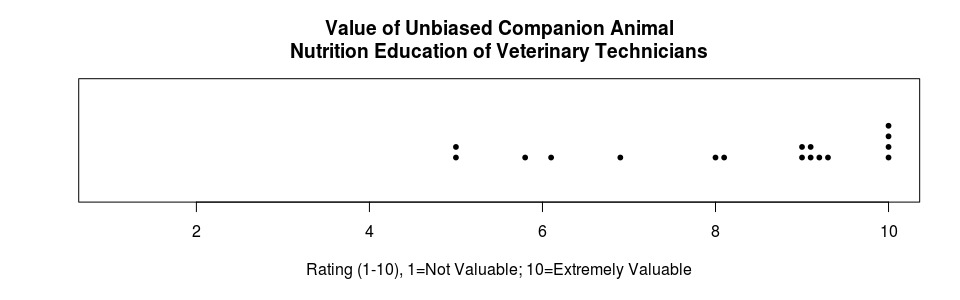
\includegraphics[width=1.0\textwidth]{Images/voucane.jpeg}
    \isucaption{Each dot represents one participant's value rating for unbiased companion animal nutrition education of veterinary technicians.}
    \label{mgraph11}
    \end{figure}
\section{Summary}
This chapter reported the results from the questionnaire with the objectives of the study as a guideline. The participants perceive themselves to be fairly knowledgeable on average in the area of companion animal nutrition, and the ratings within the specific topics related to dog and cat nutrition mostly support their perception. There was a trend as to which topics were less known by both groups. Similar results were seen with the participant familiarity of different pet food brands. Respondents were very interested in an educational program centered around dog and cat nutrition; education in nutrition was very important and very valuable to veterinary clinics in veterinary technicians.
